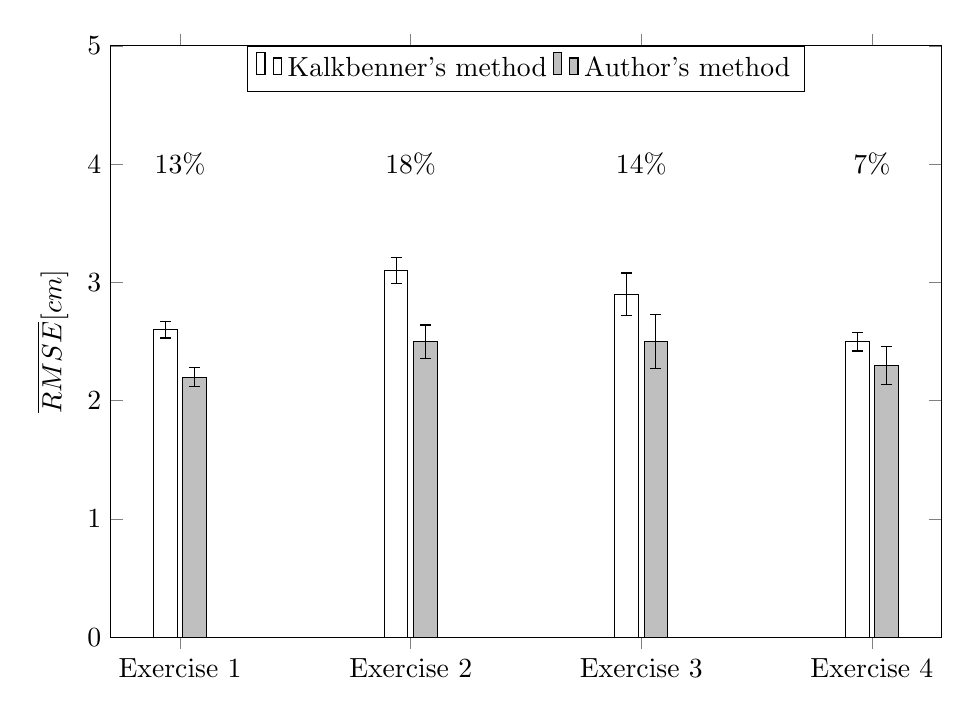
\begin{tikzpicture}
	\begin{axis}[
			ybar,
			bar width=.3cm,
			width=\textwidth,
			height=0.75\textwidth,
			legend style={at={(0.5,1)},
				anchor=north,legend columns=-1},
			symbolic x coords={ex 1,ex 2,ex 3,ex 4},
			xticklabels={Exercise 1,Exercise 2,Exercise 3,Exercise 4},
			xtick=data,
			ymin=0,ymax=5,
			ylabel={$\overline{RMSE} [cm]$},
		]
		\addplot [black,fill=white,error bars/.cd,y dir=both,y explicit] coordinates { 
			(ex 1,2.6) +- (0.0, 0.07)         
			(ex 2,3.1) +- (0.0, 0.11)
			(ex 3,2.9) +- (0.0, 0.18)  
		(ex 4,2.5) +- (0.0, 0.08) };
		\addplot [black,fill=black!25,error bars/.cd,y dir=both,y explicit] coordinates { 
			(ex 1,2.2) +- (0.0, 0.08)         
			(ex 2,2.5) +- (0.0, 0.14)
			(ex 3,2.5) +- (0.0, 0.23)  
		(ex 4,2.3) +- (0.0, 0.16) };
		\legend{Kalkbenner's method, Author's method}
		\node at (axis cs:ex 1,4){\textcolor{black}{13\%}};
		\node at (axis cs:ex 2,4){\textcolor{black}{18\%}};
		\node at (axis cs:ex 3,4){\textcolor{black}{14\%}};
		\node at (axis cs:ex 4,4){\textcolor{black}{7\%}};
	\end{axis}
\end{tikzpicture}	
